\section{Theoretical Background} \label{sec:theory}
The purpose of this chapter is to go through the preliminary wind turbine (WT) theory. (Subject to change!)

\subsection{Aerodynamics and airfoil theory} \label{sec:theory_aero}
The sun delivers energy to the earth by heating up the surface and subsequently the air of the earth. Winds occur as a result of the pressure differences that occur due to the expansion and contraction of the air. 

WTs work because they are able to convert the wind's energy into a torque in the generator which then generates electrical energy. When the wind blows over the blades of a WT it delivers some of its energy to the blade, yielding both a thrust force and torque to the blade.

In the simplest 1D momentum theory case the delivery of energy just results in a lowing of the wind speed following the rotor area. Due to mass preservation an expansion would subsequently occur as depicted in \cref{fig:betz}.
\begin{figure}[ht]
	\centering
	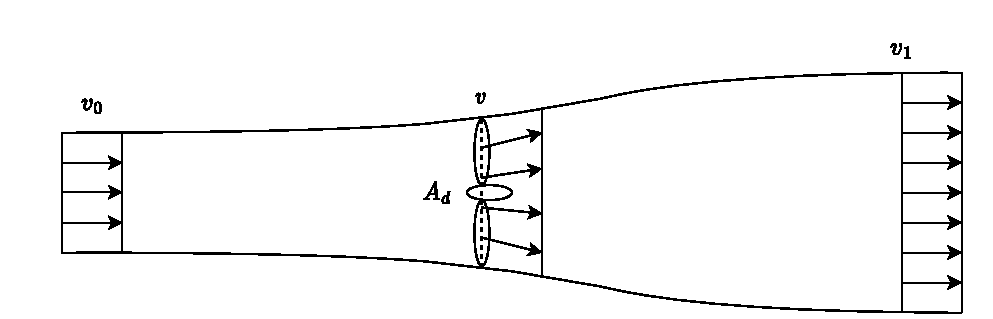
\includegraphics[width=0.8\linewidth]{Graphics/FlowThroughRotor.pdf}
	\caption{Illustration of how the wind in a control volume (CV) changes volume due to its reduction of speed}
	\label{fig:betz}
\end{figure}
The power of the \textit{free} wind $ v_0 $ can be expressed from the wind mass flow $ \dot{m} $ through a control volume:
\begin{equation} \label{eq:power}
	P = \dfrac{1}{2} \dot{m} v_0^2
\end{equation}
The flow of mass can be expressed from the air density $ \rho $, the cross sectional area $ A_d $ of the CV  at the rotor and the free wind speed $ v_0 $ as such:
\begin{equation}\label{eq:mass_deriv}
	\dot{m} = \rho A_d v_0
\end{equation}
Combining \cref{eq:power} and \cref{eq:mass_deriv} yields:
\begin{equation}\label{eq:power2}
	P_{air} = \dfrac{1}{2} \rho A_d v_0^3
\end{equation}
A \textit{power coefficient} $ C_p $ represents the percentage of the available power that is extracted from the wind:
\begin{equation}\label{eq:Cp}
	C_p = \dfrac{P_T}{P_{air}}
\end{equation}
Such that the extracted power $ P_T $ is defined:
\begin{equation}\label{eq:power_w_Cp}
	P_{T} = \dfrac{1}{2} \rho A_d v_0^3 C_p
\end{equation}
$ C_p $ is dependent on the rotor blade pitch $ \theta $ and the tip speed ratio (TSR) $ \lambda $. In the partial load region the main goal is to reach a maximum $ C_p $ by adjusting $ \theta $ and  $ \lambda $ to their optimal values:
\begin{equation}\label{eq:cp_optimal}
	C_p^\star = C_p(\theta^\star, \lambda^\star)
\end{equation}
Where $ * $ denotes the optimal value of a parameter with regards to $ C_p $. This will be further explained in \cref{sec:theory_ctrl}. The TSR is the ratio between the speed of the tip of the WT blade $ (\Omega R) $ where $ R $ is the distance from the center of the rotor and the blade tip and the incoming free wind $v_0$:
\begin{equation}\label{eq:tipspeedratio}
	\lambda = \dfrac{\Omega R}{v_0}
\end{equation}

The achievable size of $ C_p^\star $ is a matter of the WT design. The \textit{Betz limit} is the highest, optimal $ C_p $ that can be theoretically achieved and can be calculated to be:
\begin{equation}\label{eq:betzlimit}
	C_{pbetz} = 0.5962
\end{equation}
%Most often $ C_p $ is also the measure of efficiency for a WT, but a more intuitive efficiency is  calculate measure efficiency from the Betz limit extractable power:
%\begin{equation}\label{eq:efficiency}
%	\eta = \dfrac{C_p}{C_{pbetz}}
%\end{equation}

%When the air travels over the WT blade the air travels slower on one side than the other as illustrated in \cref{fig:airfoil}. Due to mass conservation the air which moves slower on the underside of the blade expands, creating a higher pressure. Likewise the air moving faster on the upper upper side contracts creating in a lower pressure. Resultingly the blade moves upwards.
%\begin{figure}[ht]
%	\centering
%	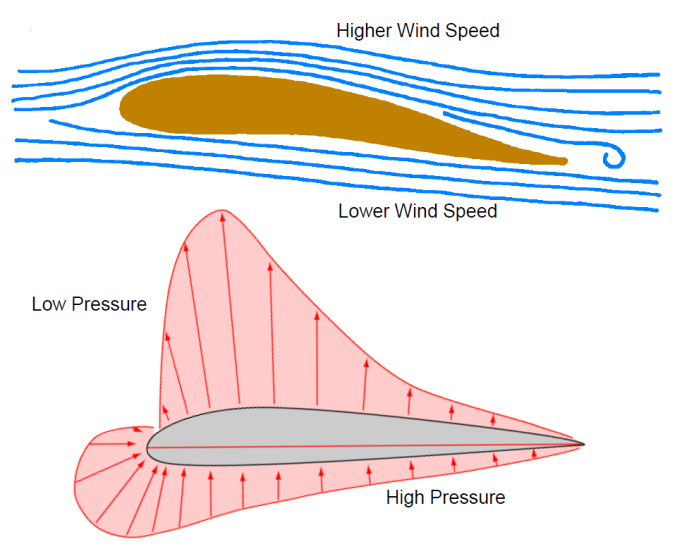
\includegraphics[width=0.5\linewidth]{Graphics/AirfoilAirflow.png}
%	\caption{Illustration of the wind speed difference between the two sides of a WT blade along with an illustration of the induced pressure difference. The result is a lifting force one the blade.}
%	\label{fig:airfoil}
%\end{figure}

Blade element momentum theory is often used to model the forces acting along WT blades. Blade element theory involves breaking a blade into small sections and determining the forces acting on each small section. In \cref{fig:blade_vel_triangle} a cross section of a WT blade can be seen. In this figure, as it is also illustrated at the rotor blade in \cref{fig:betz}, the wind velocity that hits the rotor blades is lowered indicated by the \textit{axial induction factor} $ a $. What is not observed in \cref{fig:betz} is that some of the energy of the wind also goes into driving an airstream around the back of the rotors in the opposite direction of the blade rotation, indicated by the \textit{tangential induction factor} $ a' $. This is known as \textit{swirl losses}.
\begin{figure*}[ht]
	\centering
	\subfloat[Blade cross section]{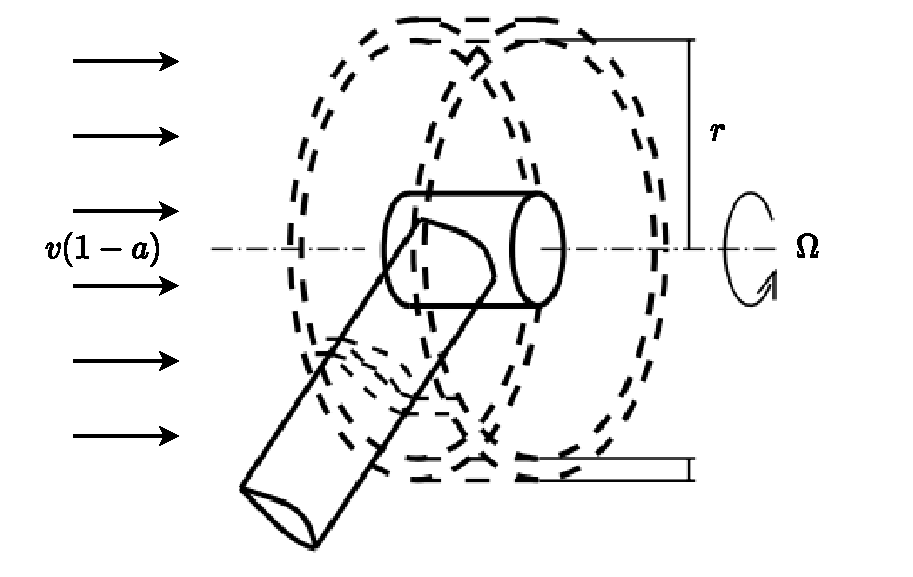
\includegraphics[width=.44\textwidth]{Graphics/RotorBladeElement.pdf}%
		\label{fig:blade_vel_triangles}}
	\hfil
	\subfloat[Velocity triangle]{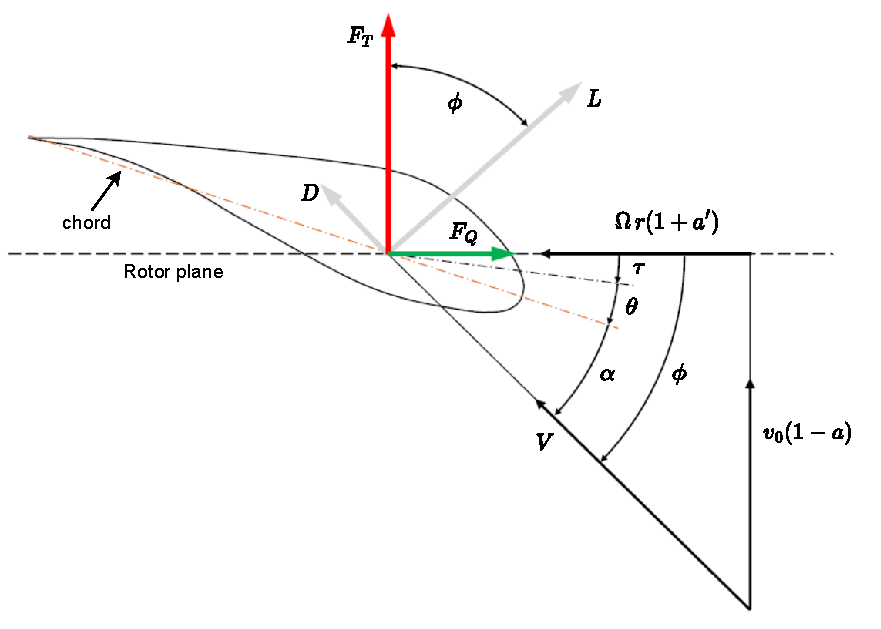
\includegraphics[width=.55\textwidth]{Graphics/BladeVelocityTriangle.pdf}%
		\label{fig:blade_vel_triangle}}
	\caption{Illustrations of a blade cross section and a velocity triangle on a blade section; \textbf{(a)} the blade cross section is made at some distance $ r $ from rotor center and rotates at a frequency $ \Omega $; \textbf{(b)} the velocity triangle acting on a cross section of a WT blade}
	\label{fig:blade_triangles}
\end{figure*}
The resulting air speed is V with an \textit{inflow angle} $ \phi $. $ F_L $ and $ F_D $ are the lift and drag forces on the blade element respectively. They are calculated from \cref{eq:lift} and \cref{eq:drag}. They include the \textit{chord length} $ c $ which is the length from the leading to the trailing edge of the blade.
\begin{align}
	F_L &= \dfrac{1}{2}\,  \rho \, V^2 c \, C_L \label{eq:lift}\\
	F_D &= \dfrac{1}{2} \, \rho \, V^2 c \, C_D \label{eq:drag}
\end{align}
The lift and drag coefficients $ C_L $ and $ C_D $ are usually extracted from table lookups which are typically found from simulations such as Xfoil
\todo{Hvad bruger Vestas til at finde $ C_L $ og $ C_D $?}. 
In a typical scenario $ C_L $ and $ C_D $ are found from the angle of attack $ \alpha $. The thrust and torque vectors $ F_T $ and $ F_Q $ are then calculated from the Pythagorean theorem as in \cref{eq:thrust} and \cref{eq:torque}
\begin{align}\
	F_T &= L \, cos(\phi) + D \, sin(\phi) \label{eq:thrust} \\
	F_Q &= L \, sin(\phi) - D \, cos(\phi) \label{eq:torque}
\end{align}
The total thrust and torque of a blade can then be calculated by integrating the above over the length of the rotor blade \cite{Knudsen2013}.


\subsection{Wind turbine control} \label{sec:theory_ctrl}
This section includes a walk-through of the main functionality of WT control. The standard WT control scheme is explained with regards to different operation regions. Furthermore the challenges presented in FOWT control are examined and some known solutions to the floating control problem are presented. 

\subsubsection{Control regions} \label{sec:theyry_ctrl_regions}
Wind turbine control is split into two main stages of control called partial load control (PLC) and full load control (FLC). In a modern variable-speed-variable-pitch (VPVP) WT such as the one at hand in this project the PLC can be further split into three subregions leaving a total of four operating regions. PLC is related to wind speed between cut-in wind speed and rated wind speed. In all three PLC regions the generator power reference is regulated with a PI controller based on a generator speed setpoint to achieve the most optimal power output. The FLC region is related to above rated wind speed to cut-out wind speed. In this region the pitch angle reference is regulated based on a generator speed set-point which is set such that a constant power output is tracked. Furthermore each of the four regions are associated with a specific wind speed range. A visualization of these operating regions can be found in figure \cref{fig:operating_regions}. The figure is simply illustrative and especially the width of the regions are out of proportion. 
\begin{figure}[ht]
	\centering
	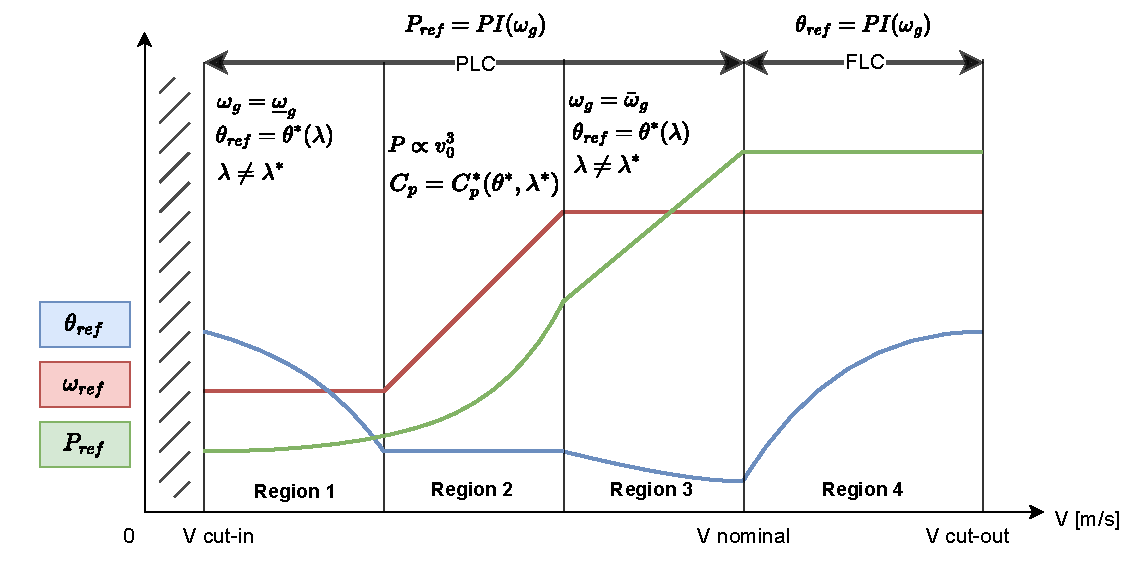
\includegraphics[width=0.9\linewidth]{Graphics/OperatingRegions.pdf}
	\caption{A visualisation of the wind turbine control operating regions. Specific wind speeds are purposefully not included since these are turbine specific. The figure is illustrative and not correctly scaled.}
	\label{fig:operating_regions}
\end{figure}
Below is a short description of the four regions focused on the parameters which are relevant to the control objective which is firstly maximisation of the turbine power output (PLC) and secondly limitation of the power output to nominal power (FLC). Below short descriptions are given to each of the WT operating regions as observed in \cref{fig:operating_regions}.
\begin{itemize}
	\item In \textbf{Region 1} the pitch angle reference is set to the optimal angle based on the tip speed ratio which in this region is \underline{not} optimal, meaning that $ C_p \neq C_p^* $ (where $ * $ denotes an optimal parameter value with regards to $ C_p $). The generator power is set by the PLC PI controller to whatever achieves the minimum rotor speed.
	\item In \textbf{Region 2} the pitch angle reference is set to the optimal angle. The tip speed ratio is optimal based on the generator speed which is controlled to the optimal value by means of the generator power. The rotor speed is proportional to the wind speed. The power output of the turbine is proportional to the third power of the wind speed. This makes sense in relation to \cref{eq:power_w_Cp}.
	\item In \textbf{Region 3} like in region 1 the angle is set to the optimal angle based on the tip speed which is not optimal. The generator power is set by the PI controller to whatever achieves the maximum allowed rotor speed. The power output of the turbine increases proportional to the wind speed.
	\item In \textbf{Region 4} the pitch angle reference is no longer set at an optimal value. It is now set by the FLC PI controller which tracks a constant nominal rotor speed reference. In FLC the power output and rotor speed is ideally close to constant while the pitch angle changes to counteract changes in wind speed.
\end{itemize}

\begin{figure}[ht]
	\centering
	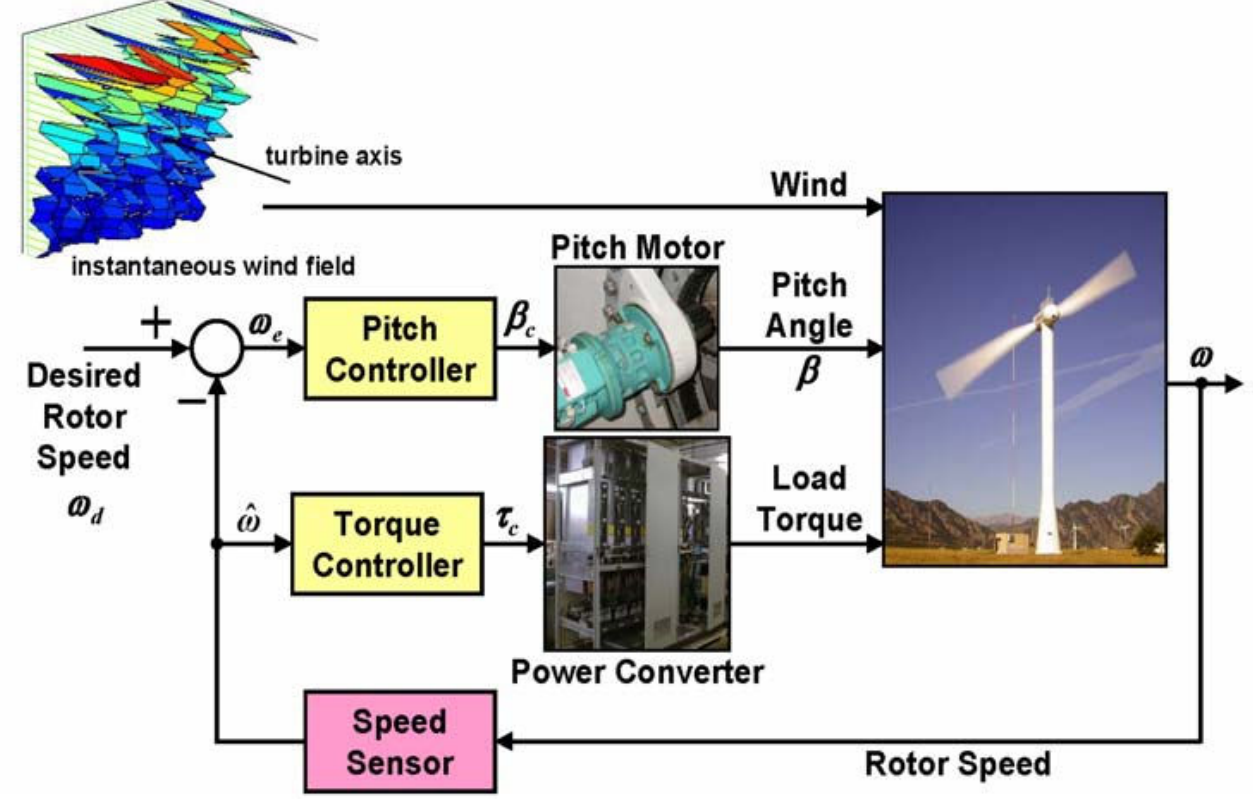
\includegraphics[width=0.7\linewidth]{Graphics/GraphicalWtController.PNG}
	\caption{An overview of the controllers. Figure from \cite{Pao2009}}
	\label{fig:controller_overview}
\end{figure}

\subsubsection{PLC}
In partial load control...\\

(inspired by PLC section from Thea):
- Cut in -> Nominal
- Power output maximation from C\_P maximation (C\_p\_max)
- Pitch angle sat at optimal value. Rotor speed regulated with power reference to optain optimal omega. (In thea's report it's defined as a torque controller)
- Classic region 2 controller: Torque controller t\_g = KOmega\^2.
- Vestas region 2 controller: PI controller with omega as input and torque OR power as output.
- PLC operating regions 1 and 3: Further explain. Lower rotor speed limit sat on region 1 to stay clear of 1P and 3P frequencies. Rated rotational speed achieved in region 3, but not rated power.
- Region 1 and 3 also uses PI controller for control of generator torque from rotor speed input (opskriv ligninger).
- Torque (or power) controller tuning (Sluggish = too slow, aggressive = instability w. regard to natural frequencies?)
- Gain scheduling is implemented by Vestas "to maintain dynamic properties throughout operating range". This gain scheduling contribution is multiplied with the generator speed error before entering the PI controller which sets a power reference. This will not be investigated further. \\

As previously mentioned the partial load control (PLC) is active from cut-in wind speed to nominal wind speed. The highest priority of the \textbf{region 2} controller is to maximize $ C_p $ such that $ C_p(\theta, \lambda) = C_p^*(\theta^*, \lambda^*) $. Two actuators could potentially be utilized to achieve this: Rotor pitch angle and generator torque. When observing a 3D plot of $ C_p(\theta, \lambda) $ such as the one in \cref{fig:cp_plot3d} it becomes apparent that maximisation of $ C_p $ will occur for specific values of $ \theta $ and $ \lambda $. In \cref{fig:cp_plot2d} the 3D plot is seen from above and thus only colours are indicators of the size of $ C_p $. Black lines are drawn on the plot which indicate a typical path from cut-in wind speed to cut-out wind speed starting in the top left corner where the tip speed ratio is very high due to the proportionally big difference between the minimum rotor speed and the low incoming wind speed and ending in the bottom right corner with the very high pitch angle. Furthermore the operating regions are drawn along the lines. It becomes obvious that all of regions 2 is centred at the $ C_p^*(\theta^*, \lambda^*) $ which is marked by a black dot in the middle of the darkest red region.
\begin{figure*}[ht]
	\centering
	
	\subfloat[$ C_p $ vs. $ \theta $ and $ \lambda $ (3D)]
	{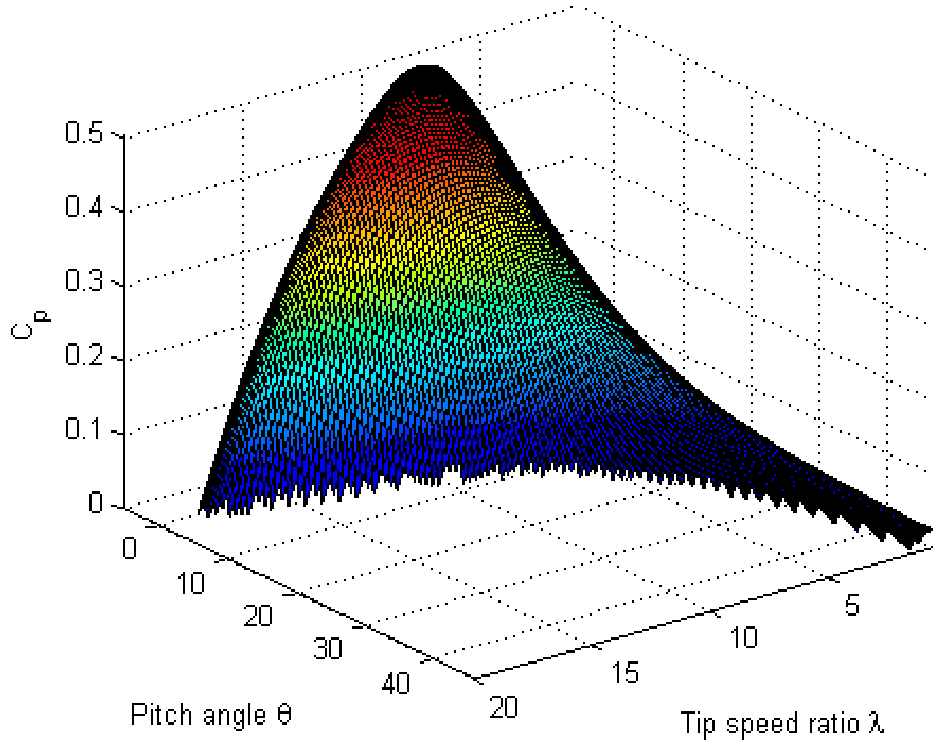
\includegraphics[width=.53\textwidth]{Graphics/Cp3dPlotV2.png}%
		\label{fig:cp_plot3d}}
	\hfil
	\subfloat[$ C_p $ vs. $ \theta $ and $ \lambda $ (2D)]
	{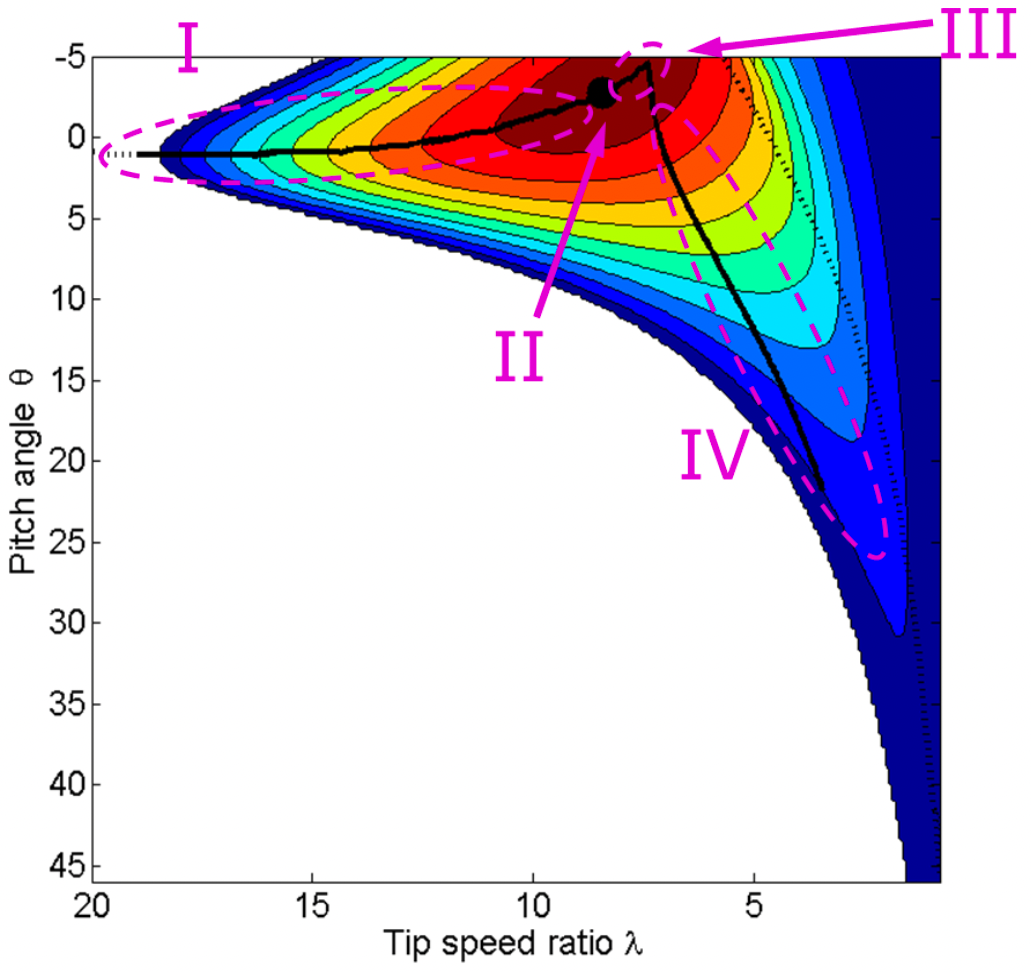
\includegraphics[width=.42\textwidth]{Graphics/Cp2dPlotRegions.png}%
		\label{fig:cp_plot2d}}
	
	\caption{Typical $ C_p $ plot drawn agains varying $ \theta $ and $ \lambda $; \textbf{(a)} 3D plot; \textbf{(b)} 2D plot where the operating regions are illustrated along the well}
	\label{fig:cp_plot}
\end{figure*}

$ \theta $ is determined from table lookups based on $ \lambda $. When $ \theta $ as such is sat at a specific values it cannot be utilized as an actuator to control the rotor speed such that $ \lambda(v_0, \Omega) = \lambda^*(v_0, \Omega^*) $ but the generator power can. Thus the primary concern is setting the generator power such that the rotor speed tracks an optimal speed based on the the wind speed. The rotor speed can be described as such:
\begin{equation}\label{eq:plc_rotor_speed}
	J \dot{\Omega} = T_r(\theta, v_0) - T_g(P_g, \omega)
\end{equation}
where $ J $ is the total inertia of all parts connected to the drivetrain, $ T_r $ the rotor torque and $ T_g $ the generator torque referred to the rotor side of the drivetrain. From this equation it becomes apparent that if $ \theta $ is sat at a fixed optimal angle the generator torque must be used to control the set-point rotor speed that makes $ C_p = C_p^* $.

While there are numerous generator torque controllers in use in the wind industry the classical WT torque controller is defined as in \cref{eq:gen_torque_ctrl} where the generator torque is calculated based on the rotor speed.
\begin{equation}\label{eq:gen_torque_ctrl}
	T_g = K \Omega^2
\end{equation}
with the \textit{generator constant} being defined as such \cite{Pao2009}:
\begin{equation}\label{eq:gen_torque_const}
	K = \dfrac{1}{2} \rho \pi R^5 \dfrac{C_{p\_max}}{\lambda^{*3}}
\end{equation}
This causes the rotor speed to tend towards the optimal rotor speed. This is more readily visible when considering \cref{eq:omega_dot}. Consider when $ \frac{C_p}{\lambda^3} $ is greater than the optimal counterpart $ \frac{C_p^*}{\lambda^{*3}} $ then $ \dot{\omega} > 0 $ which will increase $ \omega $ until an increase in the $ \lambda^3 $ term will bring the two terms closer. If $ \theta $ is sat at $ \theta^* $ then when $ \lambda^3 = \lambda^{*3} $ then $ C_p = C_p^* $ which is exactly the tracking goal.
\begin{equation}\label{eq:omega_dot}
	\dot{\Omega} = \dfrac{1}{2 J} \rho \pi R^5 \omega^2 \left( \dfrac{C_p}{\lambda^3} - \dfrac{C_p^*}{\lambda^{*3}} \right)
\end{equation}
\cref{eq:omega_dot} is derived by combining equations \cref{eq:power2}, \cref{eq:Cp}, \cref{eq:tipspeedratio}, \cref{eq:plc_rotor_speed} and \cref{eq:gen_torque_ctrl} and \cref{eq:mech_torque}.
\begin{equation}\label{eq:mech_torque}
	T_r = \dfrac{P}{\Omega}
\end{equation}
\cref{eq:mech_torque} simply states the relationship between mechanical power $ P_T $, rotor speed $ \Omega $ and torque $ T_r $\\
\smallskip
Unlike the conventional torque controller, Vestas utilizes a PI controller structure for its region 2 control. The PI controller input is the rotor speed error multiplied with a gain scheduling contribution which is dependent on the wind speed. The rotor speed reference is calculated by multiplying the wind speed with some gain $ K $. The nature of the gain $ K $ which translates the wind speed to a rotor speed reference is not further explored. The mentioned gain scheduling component is present to account for the non-linearity of the system throughout the wind operating range.

In \textbf{region 1} achieving $ C_p = C_p^* $ is disregarded in favour of maintaining a minimum rotor speed $ \underline{\omega}_g $. This is done to avoid the 3P frequency overlapping with the eigenfrequency of the system. This concept is further explored in \cref{sec:eigenfreq}. As such only $ \theta = \theta^* $ in this region.

\textbf{Region 3} is characterized by the rotor speed reaching nominal output speed $ \bar{\omega} $. Thus like in region 1 optimal $ C_p $ is disregarded to maintain the nominal rotor speed. The output power has not reached nominal output power. Thus $ \theta = \theta^* $ and $ P_g $ is sat such that $ \omega = \bar{\omega} $. As the wind increases $ C_p $ is decreased while $ P $ increases towards nominal power output. 

In both region 1 and 3 the PI controller is utilized. The rotor speed reference is simply sat at $ \underline{\omega}_g $ in region 1 and $ \bar{\omega} $ in region 3.



\subsubsection{FLC}

(inspired by FLC section from Thea):
- rated -> cut-out wind speed
- PI collective pitch controller used to set pitch blade reference based on constant rotor speed reference setpoint.
- PI controller equations
- Gain scheduling included to compensate for the pitch-dependent sensitivity (called aerodynamic gain by Thea). (In Thea it's dtau/dtheta. Vestas denotes it as dpower/dtheta). It's calculated based on pitch reference set by the FLC pitch PI controller and multiplied with the pitch reference before being input in the pitch controller system.

\subsubsection{FATD}
Introduction to the conventional fore-aft tower damper.


\medskip
\medskip
\medskip
\medskip




\begin{enumerate}
	\item The different stages of control depending on wind speed
	\item Full PLC explanation
	\item FUll FLC explanation
	\item Fore-aft tower damper (FATD) - fixed-bottom and floating
\end{enumerate}

\subsection{Eigenfrequencies and operating speeds} \label{sec:eigenfreq}
When working with WT control it is relevant to understand the relationship between the eigenfrequencies of the WT tower and the forces that excite the turbine structure.

A problem that both fixed-bottom and floating WTs have to deal with is frequency separation with regards to the natural frequencies of components and the periodic disturbances and exciting forces. Wind and waves as well as the rotating rotor will excite the tower at specific frequencies and it is important that such frequencies do not overlap with the turbine modes. Turbine towers are flexible and can as such oscillate. If a disturbance such as waves or the wind excite the WT at the same frequency as the natural frequency of the tower it will cause the tower to oscillate resulting in an increase in fatigue loads. Therefore towers are designed such that their first and second modes do not overlap with especially the 1P and 3P frequencies. 1P is the rotor rotational frequency and 3P known as the \textit{blade passing frequency} is the third multiple of 1P corresponding to the three blades of conventional horizontal WTs.
\begin{itemize}
	\item \textbf{1P} oscillations are typically activated by the periodic force acting on the WT due to the rotor and generator torque.
	\item \textbf{3P} oscillations are typically activated by the turbulence inflow going through the rotor plane which strike the rotor blades every time they pass which intuitively is three times for every full rotor rotation.
\end{itemize}

A Campbell diagram such as the one seen in figure \cref{fig:campbell} is useful for visualizing the relationship between the allowed eigenfrequency of a component and the 1P and 3P frequencies. On the x-axis is the operating frequency of the turbine in revolutions per minute [rpm]. On the y-axis is the eigenfrequency in Hz. Lines are drawn for $ \pm 5 \% $ of both 1P and 3P. For any given turbine the box drawn between the 1P and 3P regions must not touch the lines drawn for the 1P and 3P regions. It becomes apparent why a clear operating region for the turbine rotor speed is defined. For a tower whose operating region is situated between 1P and 3P: If the lower boundary of the rotational speed is lowered the allowable eigenfrequency range decreases. At some point the operating region will have to cross the 1P lines which as explained will cause resonance and as a result increased fatigue loads. \cite{Valentine2015}.
\begin{figure}[ht]
	\centering
	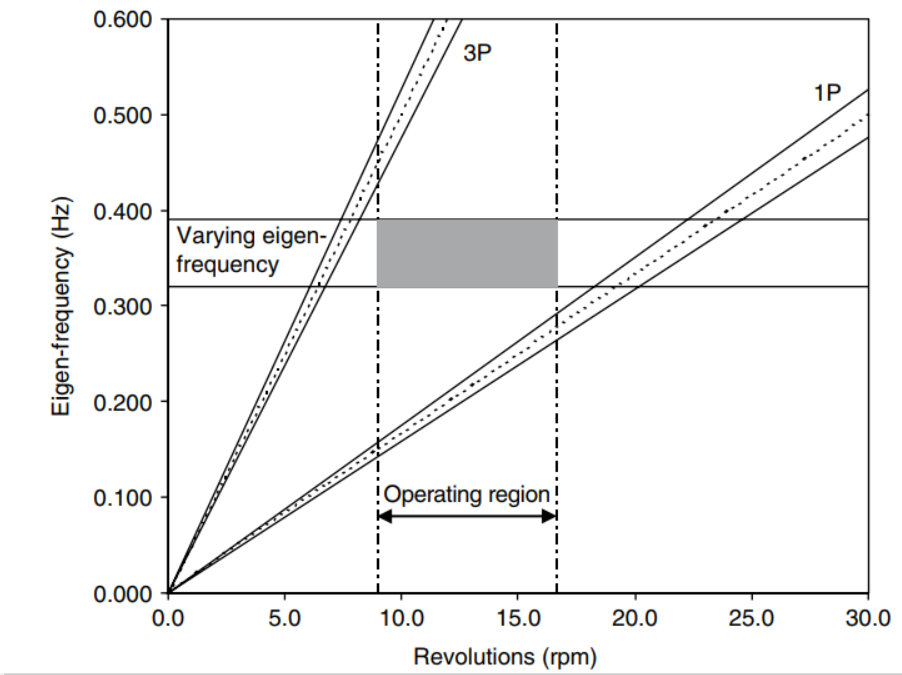
\includegraphics[width=0.5\linewidth]{Graphics/CampbellDiagram.PNG}
	\caption{The Campbell Diagram with the rotation frequency on the x-axis and the eigenfrequency on the y-axis. Figure from \cite{Valentine2015}}
	\label{fig:campbell}
\end{figure}
Modern WT towers with a \textit{soft-stiff} tower design are designed such that their first eigenfrequency ends up between the 1P and 3P frequencies and the second eigenfrequency ends up above the 3P frequency. As illustrated in the Campbell Diagram due to varying rotational frequency both 1P and 3P cover a range of frequencies. This is further illustrated in \cref{fig:1p_and3p} which furthermore highlights the possible eigenfrequency ranges of tower designs. In the diagram the natural frequency of FOWTs can be observed in frequencies way lower than 1P. The dotted line  just below the 3P frequency resembles the approximate location of the second tower mode. Its location close to 3P can cause unwanted oscillations.
\begin{figure}[ht]
	\centering
	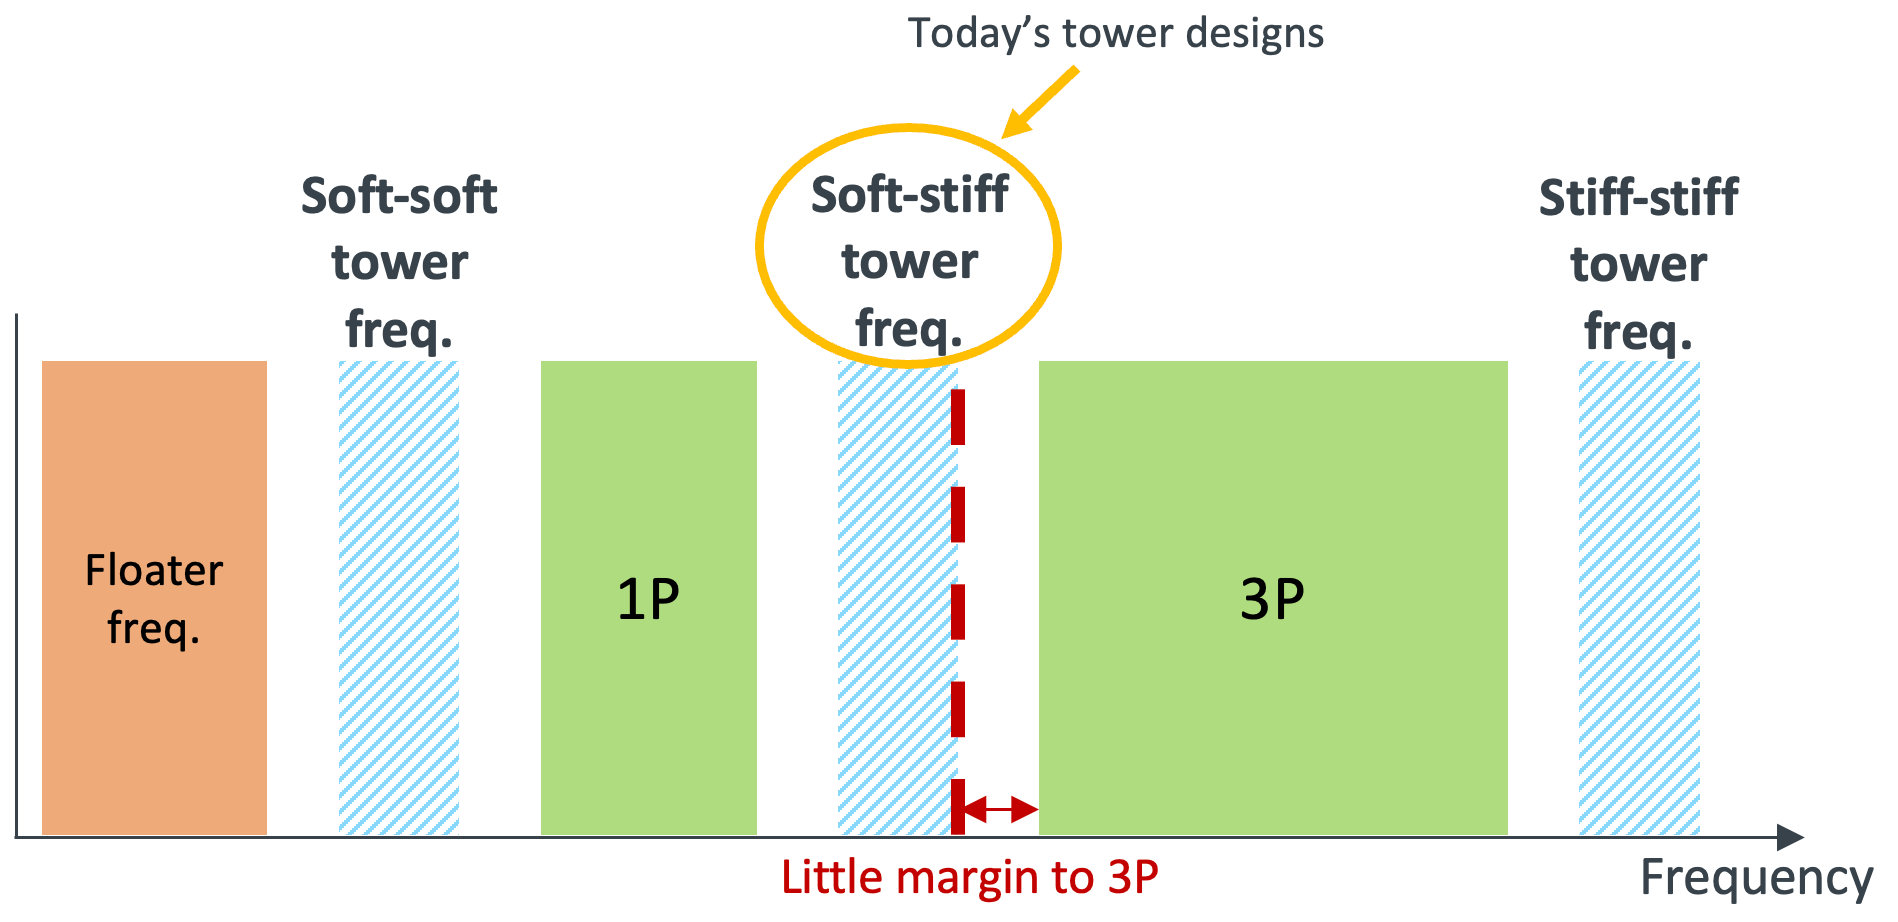
\includegraphics[width=0.7\linewidth]{Graphics/1Pand3PvsTwrStiff.PNG}
	\caption{Illustration of the frequency regions of the tower modes with different designs and for floaters as well as 1P and 3P.}
	\label{fig:1p_and3p}
\end{figure}
In \cref{fig:eigen_and_1p3p} an illustration of the tower modes of both fixed-bottom and floating WTs is found. It is apparent that the first tower mode in a conventional fixed-bottom turbine is due to the flexion of the tower while in the floating structure it is due to the tilting of the whole turbine structure. As such the conventional first tower mode of a fixed bottom turbine becomes the second mode of a floating turbine.
\begin{figure}[ht]
	\centering
	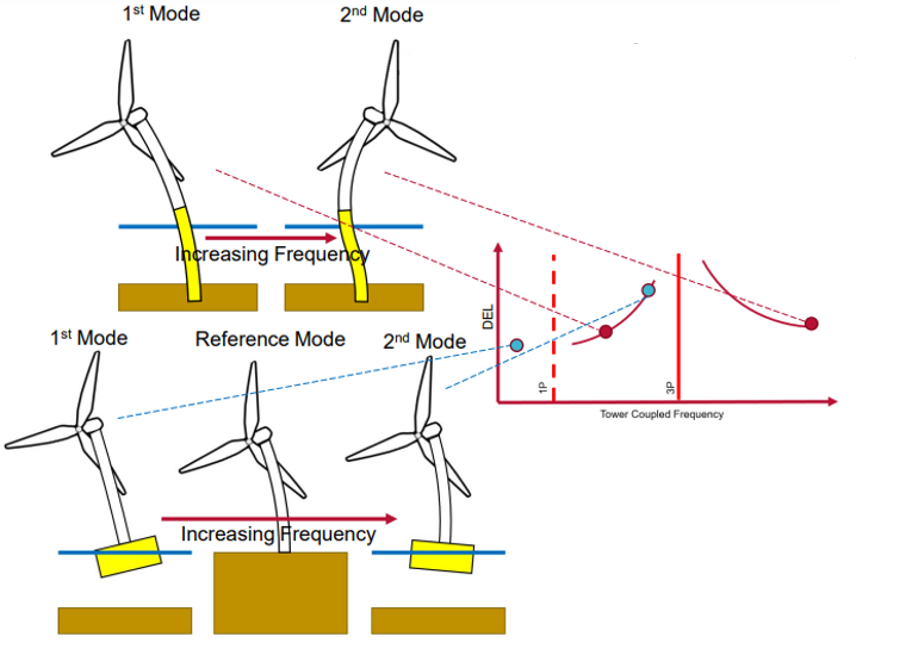
\includegraphics[width=0.7\linewidth]{Graphics/1P3PandEigenFloater.png}
	\caption{Illustration of the 1st and 2nd tower mode of both fixed-bottom and floater turbines. With floating structure the 1st mode is shiften down way past the 1P frequency}
	\label{fig:eigen_and_1p3p}
\end{figure}


\subsection{FOWT challenges and control} \label{sec:theo_fowt_challenges}
This section concerns the challenges that are persistent in FOWT design and control.



- Mention the use of a floater tuned FATD controller.
